\documentclass[conference]{IEEEtran}
\usepackage{cite}
\usepackage{amsmath,amssymb,amsfonts}
\usepackage{algorithmic}
\usepackage{graphicx}
\usepackage{textcomp}
\usepackage{xcolor}
\usepackage{placeins}           % Para controlar barreras de flotantes
\usepackage{hyperref}           % Para enlaces y \url{}
\graphicspath{{images/}}        % Ruta por defecto para las imágenes

\begin{document}

\title{Análisis y Comparación de Modelos de Clasificación para la Predicción de Churn en Clientes de Telecomunicaciones}

\author{
	\IEEEauthorblockN{Camila Pelaez\IEEEauthorrefmark{1}, Gerick Toro\IEEEauthorrefmark{1}, Cecilia Choque\IEEEauthorrefmark{1}}
	\IEEEauthorblockA{\IEEEauthorrefmark{1}Maestria en Inteligencia Artificial y Ciencia de Datos, Universidad Mayor de San Andrés, La Paz, Bolivia\\
		correos: pelaezsalazar@gmail.com, torogerick@gmail.com, cecielsachobe@gmail.com}
}

\maketitle

\begin{abstract}
	La predicción de abandono de clientes (churn) es una tarea crítica en la industria de telecomunicaciones, ya que retener clientes existentes es más rentable que adquirir nuevos. Este estudio evalúa el rendimiento de tres modelos de aprendizaje automático—Random Forest, Regresión Logística y Árbol de Decisiones—para predecir el abandono de clientes utilizando una base de datos pública disponible. El dataset utilizado incluye información demográfica, uso de servicios y detalles contractuales con el estado de Churn como variable objetivo.

	Los modelos fueron evaluados y entrenados usando métricas importantes: precisión (accuracy), exactitud (precision), sensibilidad (recall), F1-Score y área bajo la curva ROC (AUC). Los resultados muestran que la regresión logística supera a los demás modelos, alcanzando un 81.89\% de precisión, un F1-Score de 88.08\% y un AUC de 0.856.

	Los hallazgos clave sugieren que el tipo de contrato, la antigüedad del cliente (tenure) y los cargos mensuales son los predictores más influyentes en el abandono de los clientes. Este estudio resalta la utilidad del aprendizaje automático en la predicción del churn y proporciona insights para la selección de estrategias que pueden ayudar a las empresas de telecomunicaciones a retener a los clientes.
\end{abstract}

\begin{IEEEkeywords}
	Aprendizaje Automático, Árbol de Decisiones, Customer Churn, Clasificación, Modelado Predictivo, Random Forest, Regresión Logística, Telecomunicaciones
\end{IEEEkeywords}

% Nota al pie para recepción y correspondencia
\footnotetext[1]{Manuscrito recibido para revisión el 3 de mayo de 2025. Este trabajo fue desarrollado como parte del programa de Maestría en Informática de la Unidad de Posgrado de la Universidad Mayor de San Andrés (UMSA) específicamente para el módulo de Business Intelligence y Minería de Datos. Autores correspondientes: Camila Peláez, posgraduante en la Unidad de Posgrado de la Carrera de Informática, Universidad Mayor de San Andrés (correo electrónico: cpelaezsalazar@gmail.com), Gerick Toro posgraduante en la Unidad de Posgrado de la Carrera de Informática, Universidad Mayor de San Andrés (correo electrónico: torogerick@gmail.com), Cecilia Choque posgraduante en la Unidad de Posgrado de la Carrera de Informática, Universidad Mayor de San Andrés (correo electrónico: cecielsachobe@gmail.com). Repositorio del proyecto: \url{https://github.com/gerickt/Practica2_BI_M04}}

\section{Introducción}
LA industria de telecomunicaciones enfrenta un desafío significativo en la retención de clientes, donde el abandono (\emph{churn}) representa una amenaza directa para los ingresos recurrentes en las empresas. Se define \emph{churn} como el abandono del servicio por parte de un cliente, quien opta por cambiar de proveedor e irse con la competencia. Estudios previos destacan que retener a un cliente puede ser entre cinco y veinticinco veces más económico que adquirir uno nuevo, y que un incremento del 5\% en la tasa de retención de los clientes puede aumentar las utilidades de una empresa entre un 25\% y 95\% [1].

Es por eso que las empresas del sector han adoptado técnicas de inteligencia de negocios y analítica predictiva para anticipar comportamientos de abandono y ejecutar estrategias de fidelización. La predicción de \emph{churn} mediante modelos de clasificación permite identificar a clientes con mayor riesgo de desertar, facilitando intervenciones preventivas, como promociones personalizadas, mejoras en el servicio o programas de retención.

Este estudio analiza la predicción de \emph{churn} utilizando el conjunto de datos público “Telco Customer Churn”, el cual contiene información demográfica y contractual de 7,043 clientes. En este trabajo, se evalúa el desempeño de tres modelos de clasificación supervisada—Random Forest, Regresión Logística y Árboles de Decisión—. Los resultados preliminares muestran que la Regresión Logística alcanza el mayor AUC (0.856) y precisión (81.9\%), seguida por Random Forest (AUC: 0.844) y Árbol de Decisión (AUC: 0.816). Estas métricas resaltan la capacidad de los modelos para identificar patrones predictivos, como la influencia de variables contractuales, cargos mensuales y antigüedad del cliente.

Además de la comparación cuantitativa, se incluyen visualizaciones clave:
\begin{itemize}
	\item Matrices de Confusión para evaluar errores de clasificación de los modelos.
	\item Curvas ROC que validan el equilibrio entre sensibilidad y especificidad.
	\item Análisis de importancia en las variables de Random Forest y coeficientes en la Regresión Logística que aportan interpretabilidad al modelo.
\end{itemize}

\FloatBarrier
\section{Metodología}
Esta sección describe los métodos y técnicas utilizados para abordar el problema de la predicción de la pérdida de clientes en telecomunicaciones (churn). Se presenta un enfoque basado en la minería de datos, detallando los algoritmos de clasificación empleados y los conceptos fundamentales que sustentan el análisis.

\subsection{Minería de Datos y Enfoque General}
El estudio se adhiere al enfoque general de la minería de datos orientada a CRISP-DM (\emph{Cross-Industry Standard Process for Data Mining}), que abarca la comprensión del negocio y los datos, la preparación de los datos, el modelado predictivo, la evaluación de resultados y la implementación de soluciones. La minería de datos se define como el proceso de explorar grandes conjuntos de datos en busca de patrones ocultos, tendencias o relaciones significativas, empleando técnicas estadísticas y de aprendizaje automático.

En este contexto, la predicción de churn se aborda como una tarea de clasificación binaria ("el cliente se dará de baja" = Sí/No) dentro de la inteligencia de negocios (CRM). Los datos se dividieron en conjuntos de entrenamiento y prueba (train/test), y se empleó validación cruzada para garantizar la generalización. El proyecto se implementó en R (v4.x), utilizando \texttt{tidyverse}, \texttt{caret}, \texttt{rpart}/\texttt{party}, \texttt{randomForest} y funciones base de \texttt{stats}.

\subsection{Algoritmos de Clasificación Aplicados}
Se seleccionaron tres métodos supervisados para comparar su desempeño:

\subsubsection{Árbol de Decisión (Decision Tree)}
Modelo basado en una estructura de decisiones secuenciales. Mediante inducción, aprende reglas "if–then" dividiendo registros según la variable que maximiza la pureza en cada paso.

\begin{itemize}
	\item \textbf{Nodos internos:} pruebas lógicas sobre un predictor (ej., "¿Contrato = mes a mes?").
	\item \textbf{Ramas:} conducen a nuevos nodos según el resultado.
	\item \textbf{Nodos hoja:} clases de salida (ej., predicción Churn = Yes).
\end{itemize}

Se usó \texttt{rpart} (criterio Gini) y \texttt{cforest}/\texttt{ctree} de \texttt{party}. Se aplicó poda (\emph{pruning}) vía validación cruzada.

\subsubsection{Regresión Logística (Logistic Regression)}
Método clásico para clasificación binaria, modelando $P(\text{Churn}=\text{Yes})$ con una función sigmoide sobre una combinación lineal de atributos:

\begin{equation}
	\mathrm{logit}(p)=\ln\frac{p}{1-p}=\beta_0 + \sum_{i=1}^k \beta_i X_i
\end{equation}

\begin{equation}
	p=\frac{1}{1+\exp\bigl(-\bigl(\beta_0 + \sum_{i=1}^k \beta_i X_i\bigr)\bigr)}
\end{equation}

Se entrenó por máxima verosimilitud con \texttt{glm()} (familia binomial, link logit).

\subsubsection{Bosque Aleatorio (Random Forest)}
Algoritmo de \emph{ensemble} que construye múltiples árboles y vota por mayoría:

\begin{itemize}
	\item \textbf{Bootstraping:} muestreo con reemplazo para cada árbol.
	\item \textbf{Selección aleatoria de características:} aumenta la diversidad.
	\item \textbf{Votación:} clase predicha por mayoría de árboles.
\end{itemize}

Se implementó con \texttt{randomForest} en R.

\subsection{Evaluación de Desempeño}
Se compararon métricas sobre el conjunto de prueba: Exactitud (Accuracy), Precisión (Precision), Exhaustividad (Recall) y F1-Score, derivadas de la matriz de confusión. Se usó validación cruzada para estimar varianza y se exploraron curvas ROC y AUC.

\subsection{Conceptos Clave Adicionales}
\begin{itemize}
	\item \textbf{Validación Cruzada:} evaluar rendimiento dividiendo datos en múltiples subconjuntos.
	\item \textbf{Matriz de Confusión:} tabla con VP, VN, FP y FN.
	\item \textbf{Precisión, Recall y F1:} métricas clave para clases desbalanceadas.
	\item \textbf{Curva ROC y AUC:} discriminación entre clases, con AUC como resumen.
	\item \textbf{Importancia de Variables:} relevancia de predictores en el modelo.
\end{itemize}

\FloatBarrier
\section{Análisis de Resultados}
\subsection{Métricas de Evaluación}
Con el objetivo de evaluar el desempeño de los modelos de clasificación implementados, se utilizaron las métricas comunes de clasificación: precisión, exactitud, sensibilidad, F1-Score y área bajo la curva (AUC). Los resultados se presentan en la Tabla~\ref{tab:metrics}.

\begin{table}[htbp]
	\centering
	\caption{Comparación de Métricas por Modelo}
	\label{tab:metrics}
	\begin{tabular}{lccccc}
		\hline
		\textbf{Modelo}     & \textbf{Precisión} & \textbf{Exactitud} & \textbf{Recall} & \textbf{F1-Score} & \textbf{AUC} \\
		\hline
		Random Forest       & 0.7491             & 0.5182             & 0.7875          & 0.6251            & 0.8360       \\
		Regresión Logística & 0.7699             & 0.5465             & 0.7875          & 0.6452            & 0.8555       \\
		Árbol de Decisión   & 0.7666             & 0.5452             & 0.7321          & 0.6250            & 0.8082       \\
		\hline
	\end{tabular}
\end{table}

La Regresión Logística obtuvo el mayor AUC (0.8555), indicando mejor capacidad de discriminación. También destacó en F1-Score (0.6452) y precisión (0.7699), reflejando un balance óptimo entre verdaderos positivos y falsos positivos. El Random Forest mostró buen recall pero menor precisión, sugiriendo más falsos positivos. El Árbol de Decisión presentó precisión aceptable, pero recall y AUC inferiores.

\FloatBarrier
\subsection{Matrices de Confusión}
Las figuras 1, 2 y 3 presentan las matrices de confusión de cada modelo, que permiten analizar a detalle la distribución de verdaderos positivos, verdaderos negativos, falsos positivos y falsos negativos:
\begin{figure}[!htbp]
	\centering
	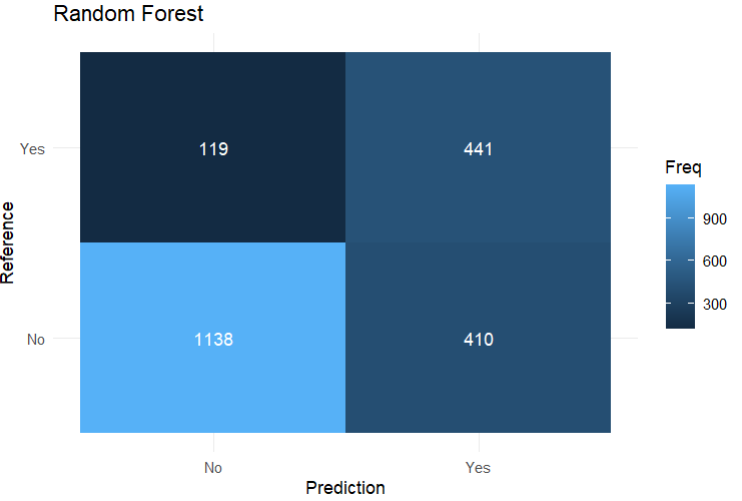
\includegraphics[width=0.8\columnwidth]{cf_randomforest.png}
	\caption{Matriz de Confusión Random Forest}
	\label{fig:cf_rf}
\end{figure}

Se puede observar que la matriz de confusión de Random Forest muestra los siguientes resultados:
\begin{itemize}
	\item Verdaderos Negativos: 1138 clientes que no abandonaron y fueron correctamente identificados.
	\item Falsos Positivos: 410 clientes que no abandonaron, pero no fueron predichos correctamente por el modelo.
	\item Verdaderos Positivos: 441 que abandonaron y fueron correctamente identificados.
	\item Falsos Negativos: 119 clientes que sí abandonaron pero fueron marcados como que no abandonaron.
\end{itemize}

\begin{figure}[!htbp]
	\centering
	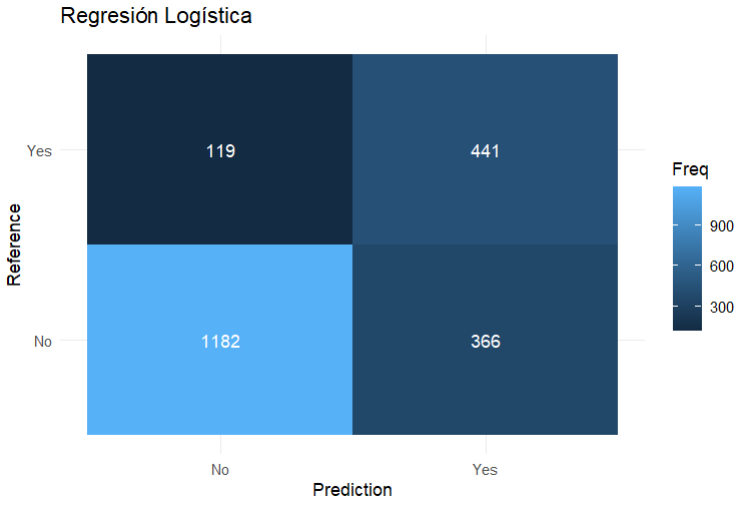
\includegraphics[width=0.8\columnwidth]{cf_logistic.png}
	\caption{Matriz de Confusión Regresión Logística}
	\label{fig:cf_lr}
\end{figure}

Se puede observar que la matriz de confusión de Regresión Logística muestra los siguientes resultados:
\begin{itemize}
	\item Verdaderos Negativos: 1182 clientes que no abandonaron y fueron correctamente identificados.
	\item Falsos Positivos: 366 clientes que no abandonaron, pero no fueron predichos correctamente por el modelo.
	\item Verdaderos Positivos: 441 que abandonaron y fueron correctamente identificados.
	\item Falsos Negativos: 119 clientes que sí abandonaron pero fueron marcados como que no abandonaron.
\end{itemize}

\begin{figure}[!htbp]
	\centering
	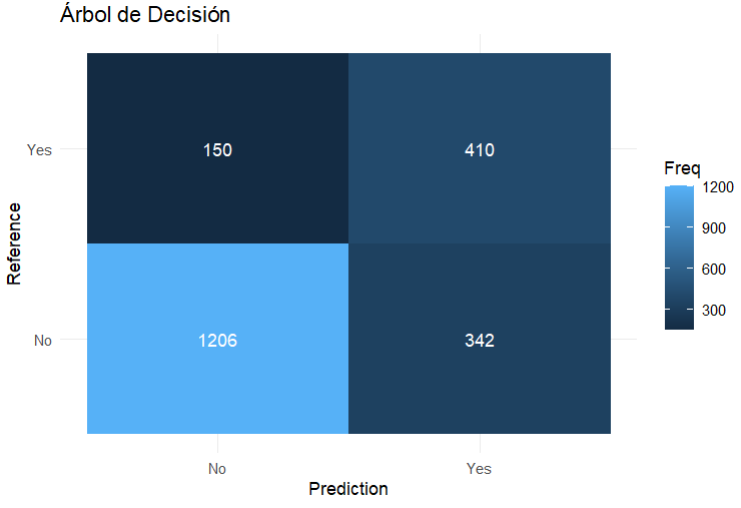
\includegraphics[width=0.8\columnwidth]{cf_decisiontree.png}
	\caption{Matriz de Confusión Árbol de Decisión}
	\label{fig:cf_dt}
\end{figure}

Se puede observar que la matriz de confusión del Árbol de Decisión muestra los siguientes resultados:
\begin{itemize}
	\item Verdaderos Negativos: 1206 clientes que no abandonaron y fueron correctamente identificados.
	\item Falsos Positivos: 342 clientes que no abandonaron, pero no fueron predichos correctamente por el modelo.
	\item Verdaderos Positivos: 410 que abandonaron y fueron correctamente identificados.
	\item Falsos Negativos: 150 clientes que sí abandonaron pero fueron marcados como que no abandonaron.
\end{itemize}

\FloatBarrier
\subsection{Curvas ROC}
La figura 4 muestra la comparación gráfica de las curvas ROC, donde el modelo de Regresión Logística obtiene el mayor AUC (0.8556), seguido del Random Forest (0.8444) y el Árbol de Decisión (0.8155).
\begin{figure}[!htbp]
	\centering
	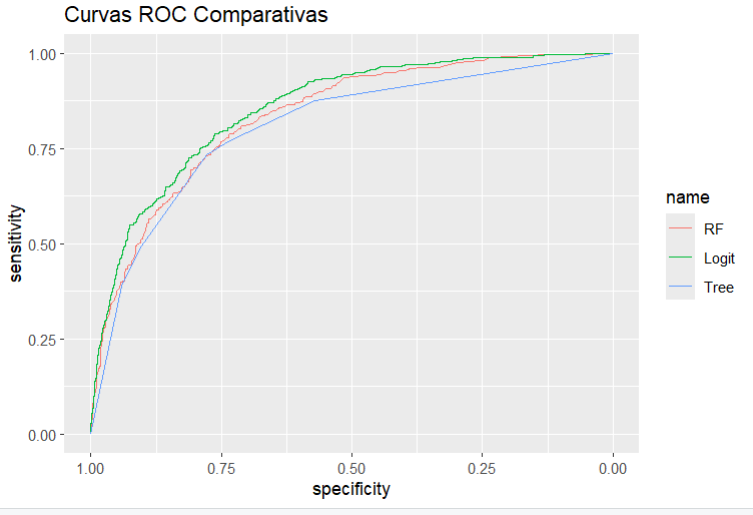
\includegraphics[width=0.8\columnwidth]{roc_curves.png}
	\caption{Curvas ROC de los Modelos de Clasificación}
	\label{fig:roc}
\end{figure}

La Regresión Logística tiene la curva más cercana al extremo superior izquierdo, confirmando de esta forma, su superioridad en distinguir entre clases. El Árbol de Decisión tiene el menor AUC, lo que indica solapamiento en las distribuciones de probabilidad.

\FloatBarrier
\section{Conclusiones}
El estudio comparativo de los tres modelos de aprendizaje automático para la predicción del churn en el sector de telecomunicaciones permitió identificar diferencias significativas en su desempeño, interpretabilidad y aplicabilidad práctica. Los hallazgos clave son:
\begin{itemize}
	\item \textbf{Regresión Logística como mejor modelo:} cuenta con mayor AUC, lo que indica una mejor capacidad para distinguir entre clientes que abandonan y los que no. Además, tiene un mejor equilibrio entre precisión y recall, reflejado en un F1-Score alto, y genera menos falsos positivos, lo que reduce costos en campañas de retención innecesarias.
	\item \textbf{Random Forest:} es útil para minimizar falsos negativos y proporciona una visualización clara de las variables críticas (tenure, \texttt{TotalCharges}, \texttt{Contract}) para predecir el churn.
	\item \textbf{Variables predictoras clave:} los contratos a largo plazo y el soporte técnico incluido reducen significativamente el riesgo de abandono.
\end{itemize}

\FloatBarrier
\section{Aprendizajes y Recomendaciones}

Los modelos muestran que, para reducir el abandono es importante priorizar a los clientes que cuentan con contratos mensuales y servicios de fibra óptica, ya que son los más propensos a abandonar. Se pueden ofrecer incentivos para migrar a contratos más a largo plazo y paquetes que combinen más de un servicio.

Es importante fortalecer la retención con el soporte técnico proactivo para clientes con muchas incidencias y facturación sobre todo, vía cheque electrónico.

Los modelos de análisis predictivo son esenciales para transformar datos en decisiones accionables. En el estudio, demostraron su capacidad para identificar patrones ocultos en el comportamiento de los clientes, como la correlación entre las variables importantes. La regresión logística se convirtió en el aliado para el diseño de estrategias de retención confiables. 

\FloatBarrier
\section{Apéndice}
\subsection{Análisis Complementario}

\begin{figure}[!htbp]
	\centering
	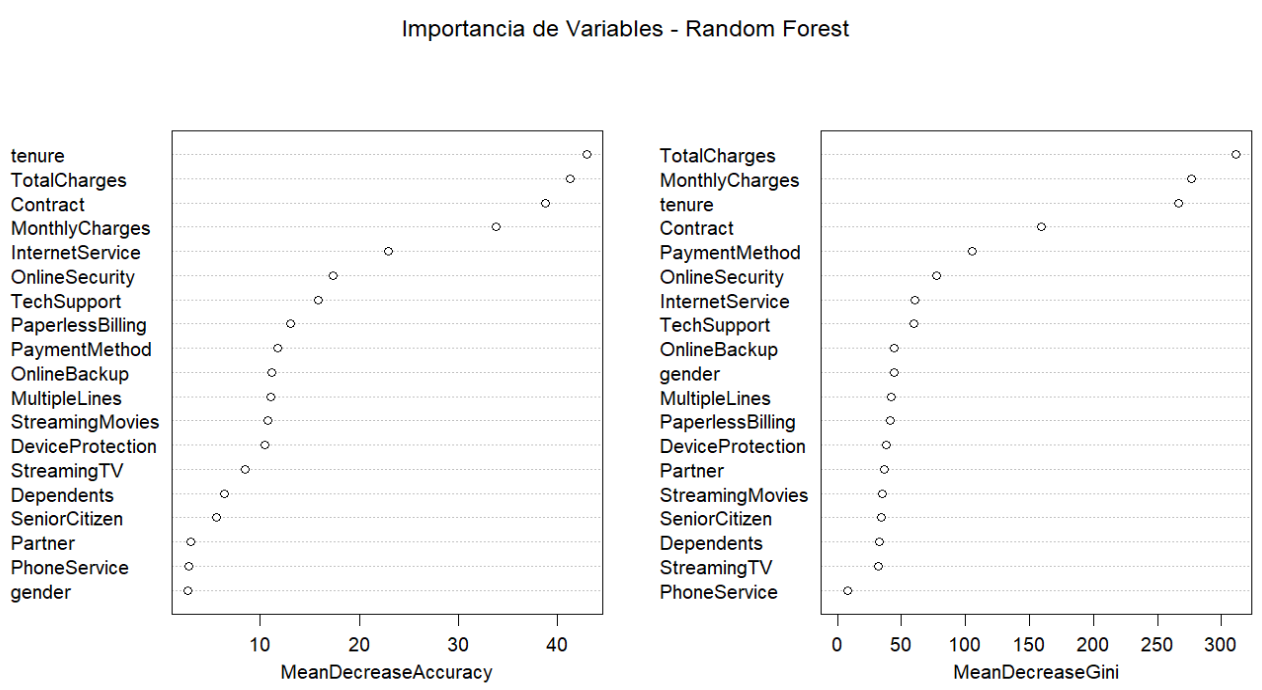
\includegraphics[width=0.9\columnwidth]{variable_importance.png}
	\caption{Importancia de las Variables de Random Forest}
	\label{fig:varimp}
\end{figure}

Se utilizaron dos métricas importantes:
\begin{itemize}
	\item \textbf{Mean Decrease Accuracy}: Cuánto disminuye la precisión del modelo si se elimina una variable.
	\item \textbf{MeanDecreaseGini}: Cuánto reduce la pureza de los nodos al usar una variable para dividir los datos.
\end{itemize}

Las variables más importantes según ambas métricas son \texttt{tenure}, \texttt{TotalCharges}, \texttt{Contract}, \texttt{MonthlyCharges}, \texttt{InternetService}, \texttt{PaymentMethod}, \texttt{OnlineSecurity} y \texttt{TechSupport}.

\begin{figure}[!htbp]
	\centering
	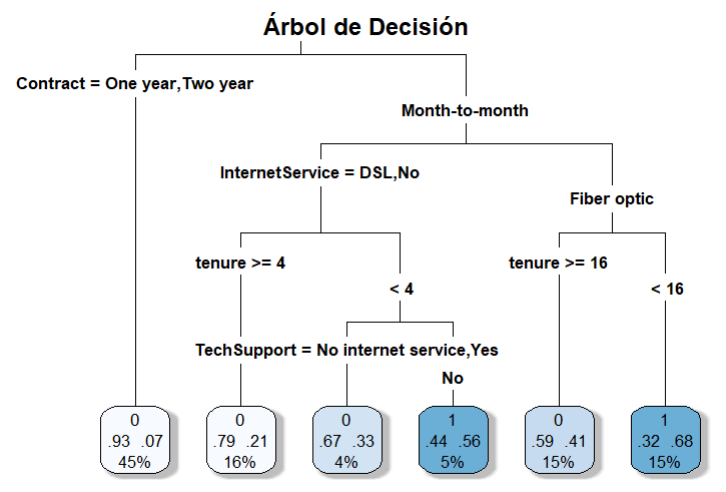
\includegraphics[width=0.9\columnwidth]{decision_tree.png}
	\caption{Visualización del Árbol de Decisión}
	\label{fig:dectree}
\end{figure}

La primera división se realizó según el \texttt{Contract}, donde contratos largos sugieren menor riesgo de churn y contratos mensuales indican mayor riesgo, especialmente si el \texttt{InternetService} es fibra óptica y no cuentan con \texttt{TechSupport}. Clientes con menor \texttt{tenure} muestran también menor riesgo de abandono.

\begin{figure}[!htbp]
	\centering
	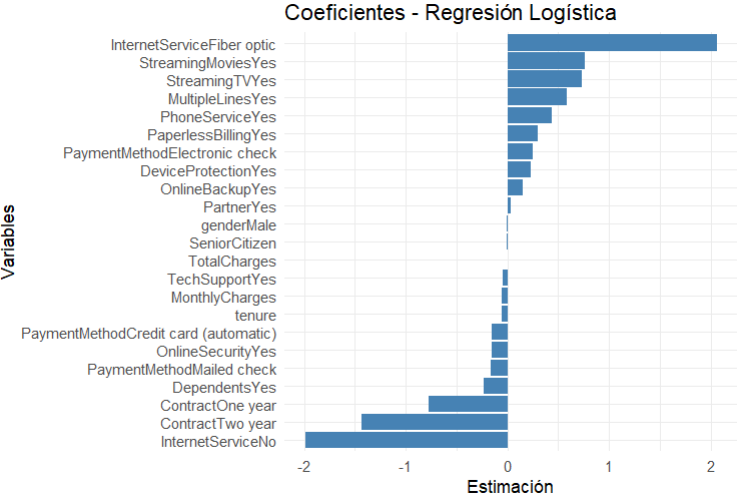
\includegraphics[width=0.9\columnwidth]{logistic_coef.png}
	\caption{Coeficientes Estimados de Regresión Logística}
	\label{fig:logcoef}
\end{figure}

Se observa que clientes con \texttt{InternetService} de fibra óptica o que pagan con \texttt{PaymentMethod} “Cheque Electrónico” son más propensos a cancelar, mientras que quienes tienen contratos largos y sin servicio de Internet presentan menor propensión.

\FloatBarrier
\section{Referencias}
\begin{thebibliography}{1}
	\bibitem{saleh2023} S. Saleh y N. Alsharif, “Customer retention and churn prediction in the telecommunication industry: a case study on a Danish university,” Discover Applied Sciences, vol. 1, Art. no. 30, 2023. Disponible en línea: Springer Link.
\end{thebibliography}

\end{document}
